\documentclass{article}
\usepackage[utf8]{inputenc}
\usepackage[a4paper,margin=1.5in]{geometry}
\setlength{\parindent}{0pt}

%\title{Using BEAST to Reconstruct Pathogen Spread Incorporating Individual Travel Histories}
\title{Bayesian Phylogeographic Analysis Incorporating Predictors and Individual Travel Histories in BEAST}
%\title{Reconstructing Pathogen Spread by Incorporating Individual Travel Histories in BEAST}
\author{Samuel L. Hong}
%GB: other authors: MAS, GB, PL? anyone else?

\usepackage{graphicx}
\usepackage{url}
\usepackage{mathabx}
\usepackage{sectsty}
\allsectionsfont{\normalsize\bfseries}
\usepackage{multicol}
\usepackage{changepage}
\usepackage{breakcites}
\usepackage{subcaption}

\captionsetup{justification=justified,singlelinecheck=false}

\newcommand{\ann}[1]{
\begin{adjustwidth}{0.5cm}{}
\it{#1}\\
\end{adjustwidth}}

\newcommand{\code}[1]{
{\upshape\ttfamily{#1}}}

\begin{document}

\maketitle

\begin{abstract}
\begin{adjustwidth}{0.5cm}{0.5cm}
Advances in sequencing technologies have tremendously reduced the time and costs associated with sequence generation, making genomic data an important asset for routine public health practices. Within this context, phylogenetic and phylogeographic inference has become a popular method to study disease transmission.
In a Bayesian context, these approaches have the benefit of accommodating phylogenetic uncertainty and popular implementations provide the possibility to parameterise the transition rates between locations as a function of epidemiological and ecological data to reconstruct spatial spread while simultaneously identifying the main factors impacting the spatial spread dynamics.
Recent developments enable to make use of additional metadata in the form of travel history data of infected individuals in the reconstruction of pathogen spread, offering increased inference accuracy and mitigating sampling bias.
We here describe a detailed workflow on how to reconstruct the spatial spread of a pathogen through Bayesian phylogeographic analysis in discrete space using these novel approaches implemented in BEAST.
The individual protocols focus on how to incorporate molecular data, covariates of spread and individual travel history data into the analysis. 
\end{adjustwidth}
\end{abstract}

\section*{INTRODUCTION}

Bayesian Evolutionary Analysis Sampling Trees (BEAST) \cite{beast110} is a software package that provides a general framework for phylogenetic inference and evolutionary hypothesis testing using molecular sequence data \cite{beastOG,beast17,beast110}.
As such, BEAST employs a combination of different types of models (including but not limited to molecular clock models, coalescent models and substitution models) to infer time-calibrated phylogenetic trees from an alignment of time-stamped sequences.
Phylogeographic analyses based on simple ancestral trait reconstruction models incorporate sampling locations as additional data.
For discrete locations, the trait evolution process, modelled as a continuous-time Markov chain process, can be parameterised in terms of covariates to help uncover the key factors that facilitate or prevent the spread of a pathogen.
Inference under these models is performed through Markov chain Monte Carlo (MCMC) sampling and the likelihood evaluations make use of BEAGLE, a high-performance computational library for statistical phylogenetics \cite{beagle3}.
BEAST is widely used in the field of phylodynamics and molecular epidemiology of infectious disease as it allows obtaining insights from molecular data through an expanding array of statistical models and estimation procedures. \\

Here, we focus on Bayesian phylogeographic inferences that aim to answer the question of ``how did an epidemic spread through space and time?" through jointly reconstructing the evolutionary and geographical history of a pathogen population in the form of (geographically) annotated time-scaled phylogenies.
Specifically, we focus on the discrete model in which transition rates are function of potential predictors of spatial spread according to a simple generalized linear model (GLM).
Such an approach has previously enabled researchers to, for example, assess the impact of air travel on the global spread of influenza \cite{glm}. 
Importantly, the GLM formulation generally also offers a sparser parameterization of the spatial transition process as it avoids having to estimate all estimate all pairwise transitions rates, which scale quadratically with the number of locations and can be difficult to inform. \\
%PL: deleted the sentence below to avoid redundnacy
%Because of the flexibility of this framework, Bayesian phylogeographic analyses in BEAST have enjoyed wide success in uncovering the origins of viral lineages \cite{hiv} and characterizing pathogen spread to inform public health response \cite{ebola}. 


%PL: the text below is also a bit repetitive partially due to some edits. I expanded a bit on the TH instead
%BEAST constitutes a popular software package to model the spatial spread of a pathogen between discrete locations using discrete trait analysis (DTA) through Bayesian inference.
%DTA estimates the probability of pathogen transmission between two locations using a continuous--time Markov chain (CTMC) model analogous to those used for characterising nucleotide substitution probabilities \cite{dta}.
While phylogeographic analyses incorporate the location of sampling as a discrete trait associated with each pathogen genome, it is possible that sampled patients had recently travelled to different locations. 
In fact, during epidemics travellers may be specifically screened if they return from areas with high incidence. This has been the case for SARS-CoV-2 and it has motivated the development of model extensions that incorporate the specific times and locations of travel \cite{travhist}. This may be particularly useful for capturing diversity in the locations that remain under-sampled, and as such, it can mitigate bias associated with disparate sampling efforts. 
These are important considerations because the computationally convenient ancestral reconstructions are highly sensitive to sampling bias. \\


We here provide four related protocols to reproduce the travel history-aware phylogeographic reconstructions performed in \cite{travhist}.
Protocol 1 introduces the GISAID database \cite{gisaid} (\url{https://www.gisaid.org/}) and provides the required steps to construct a SARS-CoV-2 multiple sequence alignment from this database.
In Protocol 2, we provide instructions on how to set up a discrete state phylogeographic inference under the GLM parametrisation using BEAUti, a GUI tool shipped with BEAST.
Protocol 3 introduces an automated script to modify a BEAUti-generated XML file to incorporate travel history data, which can subsequently be run using BEAST.
Finally in Protocol 4, we guide the user through the process of visualising individual spatial dispersal histories from the posterior distribution of trees estimated by BEAST.


\section*{PROTOCOL 1: CREATING A SARS-CoV-2 MSA USING SEQUENCES FROM GISAID}

The first step in any phylogenetic or phylogeographic analysis is to obtain a high-quality multiple sequence alignment (MSA).
The largest publicly accessible repository of genomes is available through the GISAID database.
The GISAID initiative provides a platform to openly share genomic data of influenza viruses as well as SARS-CoV-2 under specific rules \cite{gisaid}.
Access to the database is free (\url{https://www.gisaid.org/registration/register/}), but requires the user to register and agree to GISAID's terms of use in order to obtain access.\\

This protocol describes how to construct a SARS-CoV-2 MSA from sequences downloaded from GISAID. Specifically, we will construct an alignment for the 282-taxa dataset analysed in \cite{travhist}. 

\subsection*{\textbf{\textit{Necessary Resources}}}
\subsubsection*{Hardware}
\hspace{0.5cm}Standard computer running Linux, MacOS or Windows 10. 

\subsubsection*{Software}
\hspace{0.5cm}A modern web browser (Google Chrome and Mozilla Firefox recommended).

\hspace{0.5cm}The latest MAFFT \cite{mafft} version (v7.453 used in this protocol) 

\hspace{0.5cm}The latest Aliview \cite{aliview} version (v1.26 used in this protocol).

\hspace{0.5cm}A terminal emulator running a standard Unix shell. \\
\ann{For Windows, a BASH shell can be installed through the Windows Subsystem for Linux. For more information, see \url{https://docs.microsoft.com/en-us/windows/wsl/}}

\subsubsection*{Files}
\hspace{0.5cm}A list of GISAID accession numbers/identifiers. 

\hspace{0.5cm}A FASTA file with the untranslated regions (UTR) from the SARS-CoV-2 reference genome sequences.\\
\ann{Example files can be found at \\
\url{https://github.com/hongsamL/travHistProtocol/tree/main/files/Protocol1}} 

1. Search and download the desired sequences in the GISAID database \\

Log on to GISAID and click on \code{EpiCoV\textsuperscript{TM}}'s Browse tab to access a table with all available SARS-CoV-2 sequences in the database. To bulk download sequences by accession ID, click on the Fulltext{\Large $\blacktriangleup$} button, paste your comma-separated list of accessions (see Files for an example) in the search box, and download the FASTA sequences using the download button (Figure \ref{fig:GISAID}). In this example, we will save the sequences in a file called \code{gisaid\_selection.fasta}.\\ 

\ann{We can also use the \code{EpiCoV} Browse portal to download a custom selection of genomes. On the header section of the table you will see multiple search fields and drop-down menus to filter sequences according to different criteria.}


\begin{figure}[!ht]
    \centering
    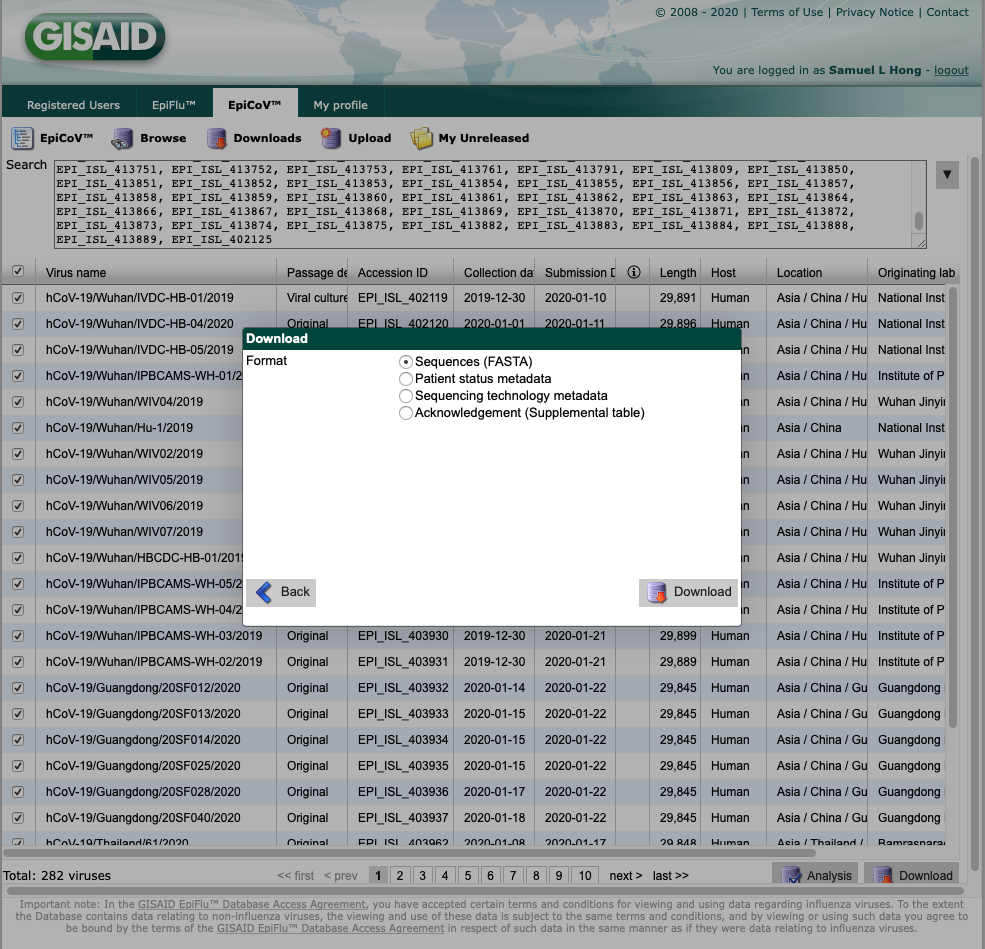
\includegraphics[width=0.99\textwidth]{figs/gisaid_screenshot.png}
    \caption{EpiCoV GISAID portal. Here, we search for all 282 sequences analysed in \cite{travhist}, and download them by selecting the checkbox on the left of the table and pressing the download button. We can also download metadata for the sequences and the corresponding GISAID acknowledgement table using the same approach.}
    \label{fig:GISAID}
\end{figure}


2. Remove whitespace from the FASTA file 
\begin{verbatim}
sed -i.bkp "s/ /_/g" gisaid_selection.fasta 
\end{verbatim}

\ann{To avoid potential issues when parsing the FASTA headers with whitespaces (e.g. in country names), we replace all whitespace in the file with underscores using \code{sed}.  We use the \code{-i} flag to find and replace the file in-place while keeping a backup of the original file.}

3. Align the sequences using MAFFT
\begin{verbatim}
cat utr.fasta >> gisaid_selection.fasta
mafft --thread -1 --nomemsave gisaid_selection.fasta > gisaid_aln.fasta
\end{verbatim}

\ann{To remove potential sequencing errors in the error-prone 5' and 3' ends of the virus, we include the reference sequences for the 5' and 3' UTRs of the SARS-CoV-2 genome (see example files).
We do this so that we can later trim these regions from the final alignment.
We concatenate these sequences to the FASTA file containing our genomes of interest, and align all sequences using MAFFT.} %GB: how about mentioning here how many positions are in this alignment (i.e. after running MAFFT)? could be useful for people going through the steps; alternatively, how about providing this alignment in supplementary material? %SH: We can't provide the alignment because we are not allowed to share GISAID data outside of GISAID per their rules . 

4. Manually trim UTRs in the MSA using Aliview\\

In Aliview, visually identify the UTR sequences and manually select the corresponding sites. Remove the selected sites using the Edit menu. %GB: I think a screenshot (start of the alignment will suffice) could be useful here; if it's visually more appealing (i.e. depending on how it plays out with figure placement within the text), please also include a screenshot of the situation at the end of the alignment %SH done
Remove the now-empty reference sequences and save the trimmed MSA (Figure \ref{fig:aliview}).\\ %GB: it may also prove useful to explicitly mention here how many sites were trimmed at both ends of the alignment %SH: Added in the figure caption

\begin{figure}[!ht]
    \centering
    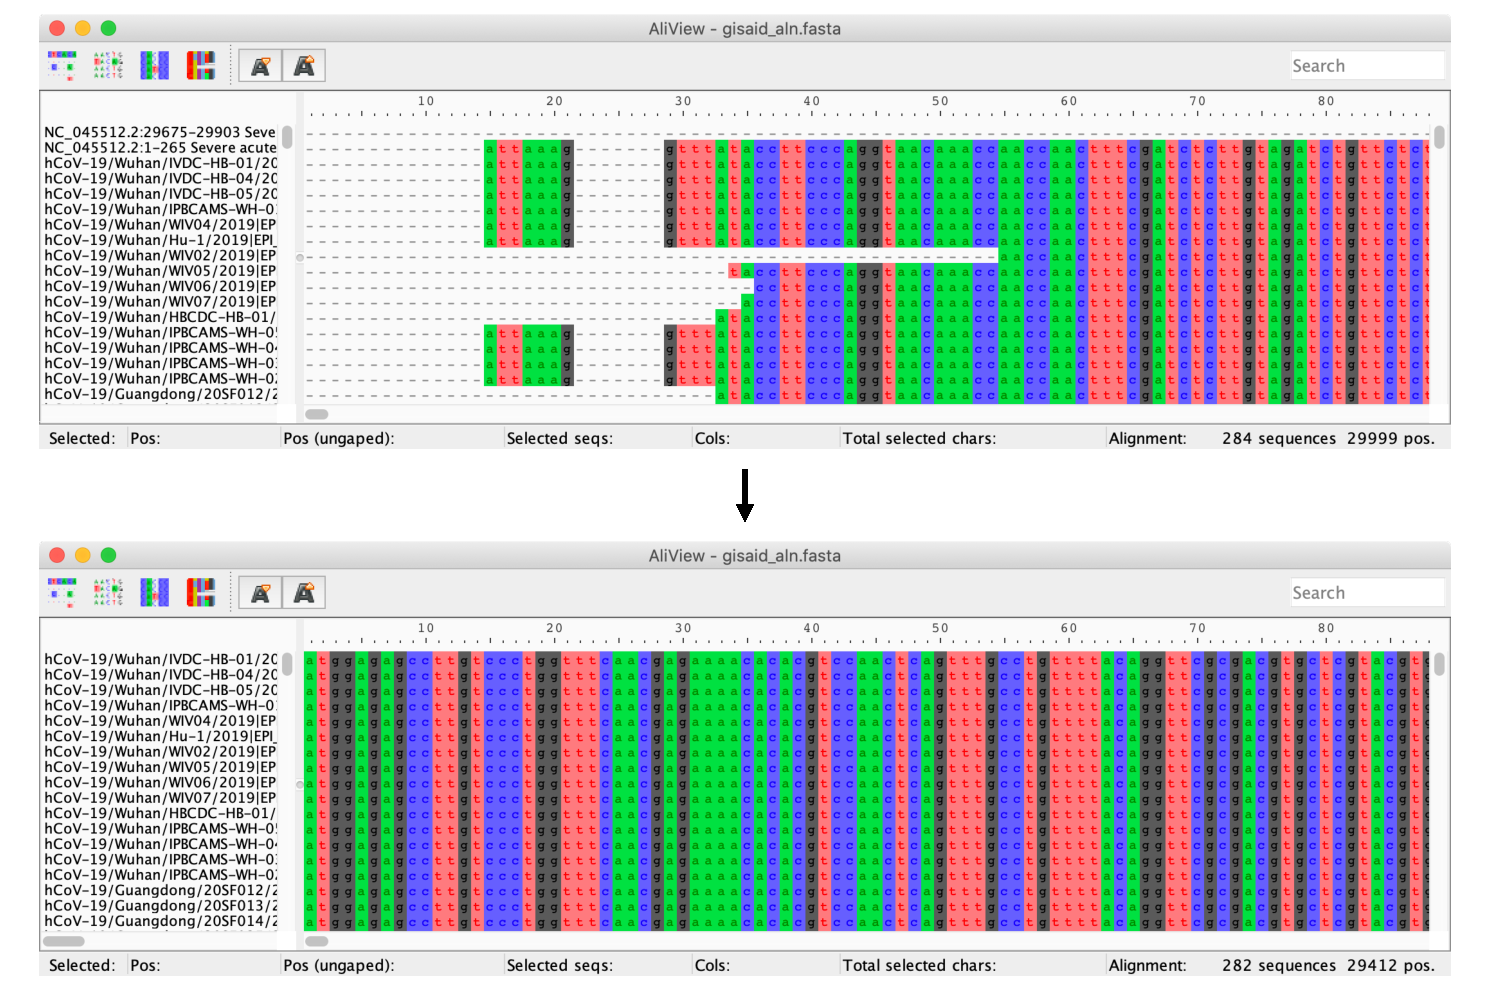
\includegraphics[width=0.99\textwidth]{figs/aliview.pdf}
    \caption{Alignment visualizations in Aliview before (top) and after (bottom) trimming the 5' and 3' UTR regions. Here, we remove a total of 286 sites on the 5' side and 301 sites on the 3' side, bringing the alignment length to 29,412 sites.}
    \label{fig:aliview}
\end{figure}


\section*{PROTOCOL 2: SETTING UP A DISCRETE TRAIT PHYLOGEOGRAPHIC RECONSTRUCTION IN BEAUTI}

Performing Bayesian phylogeographic inference while accommodating individual travel history data constitutes an extension of traditional Bayesian DTA \cite{dta} available in BEAST.
BEAUti is an interactive graphical application that enables to design the analysis you want to perform in BEAST and generates an XML file that will serve as the input file for BEAST.
This XML file contains all the required data, the models (and priors) that were selected in BEAUti, and the computational settings which will be used to run the MCMC algorithm that will collect samples of all relevant parameters (including the phylogenetic tree with annotated ancestral locations) from the joint density. \\ 

This protocol describes how to set up a DTA analysis with a generalized linear model (GLM) extension to simultaneously reconstruct spatiotemporal history and test the contribution of potential predictors of spatial spread using BEAST \cite{glm}.
Such an approach parameterizes each rate of among-location movement in the phylogeographic model as a log linear function of the provided predictors.
In this example, we will use the MSA generated in Protocol 1 to set up a DTA+GLM phylogeographic reconstruction using a flight connectivity matrix and a great-circle distance matrix as covariates (but see \cite{travhist} for more detailed information).


\subsection*{\textbf{\textit{Necessary Resources}}}
\subsubsection*{Hardware}
\hspace{0.5cm}Standard computer running Linux, MacOS, or Windows. 

\subsubsection*{Software}
\hspace{0.5cm}Latest BEAUti version (v1.10.5)

\subsubsection*{Files}
\hspace{0.5cm}Multiple sequence alignment

\hspace{0.5cm}Tab-delimited metadata file

\hspace{0.5cm}Covariate matrices in CSV format\\

\ann{Example metadata and covariate files available at\\
\url{https://github.com/hongsamL/travHistProtocol/tree/main/files/Protocol2}} 

1. Import the MSA into BEAUti\\

Load the MSA into BEAUti by selecting Import Data from the File menu (do not use Open\ldots). You can also do this by dragging the FASTA file into the Partitions panel.\\

2. Specify the sampling dates for the tips\\

Select the Tips tab and check the ``Use tip dates" box. By default, all taxa will show as having a date of zero (i.e. all sequences were sampled at the same time in the present).
To specify each sampling date, select ``Import Dates" and load the metadata file. This metadata file contains a tab separated table mapping the FASTA header of each sequence in the alignment with the corresponding sampling date. When loading the file, select the ``Parse calendar dates with variable precision" option.
This allows for taxon dates to have different degrees of resolution (e.g. year-month-day vs. year-month). We estimate the sampling dates for those sequences without day-level resolution by selecting ``Sampling uniformly from precision'' in the ``Tip date sampling" menu at the bottom of the table. \\

\ann{It is also possible to specify the sampling dates without using a metadata file. This is done by parsing the FASTA headers of each sequence. To do this, click on ``Parse Dates", and specify the rules for delimiting the date from all taxon labels. For an example of what this looks like, see \cite{skyprot} Figure 2a.}

3. Specify the sampling location of each taxon as a discrete trait\\

Click on the Traits tab.
To associate each taxon with a sampling location, click on ``Import traits" and select the metadata file (Figure \ref{fig:location}).
This will create a new trait for each column on the metadata file. Delete all non-relevant traits by clicking on the ``-" button at the bottom-left of the page (keep only the ``location'' trait for this example). Select the desired trait and click on ``create partition from trait". A new partition containing the trait data will be created under the Partitions tab.\\

\ann{It is also possible to add a discrete trait without using a metadata file. This is done by parsing the FASTA headers of each sequence. To do this, click on ``Add Trait" to create a new trait with a corresponding data partition. Select all taxa and click on ``Guess trait" values to parse the trait values from the taxon labels.}

\begin{figure}[!ht]
    \centering
    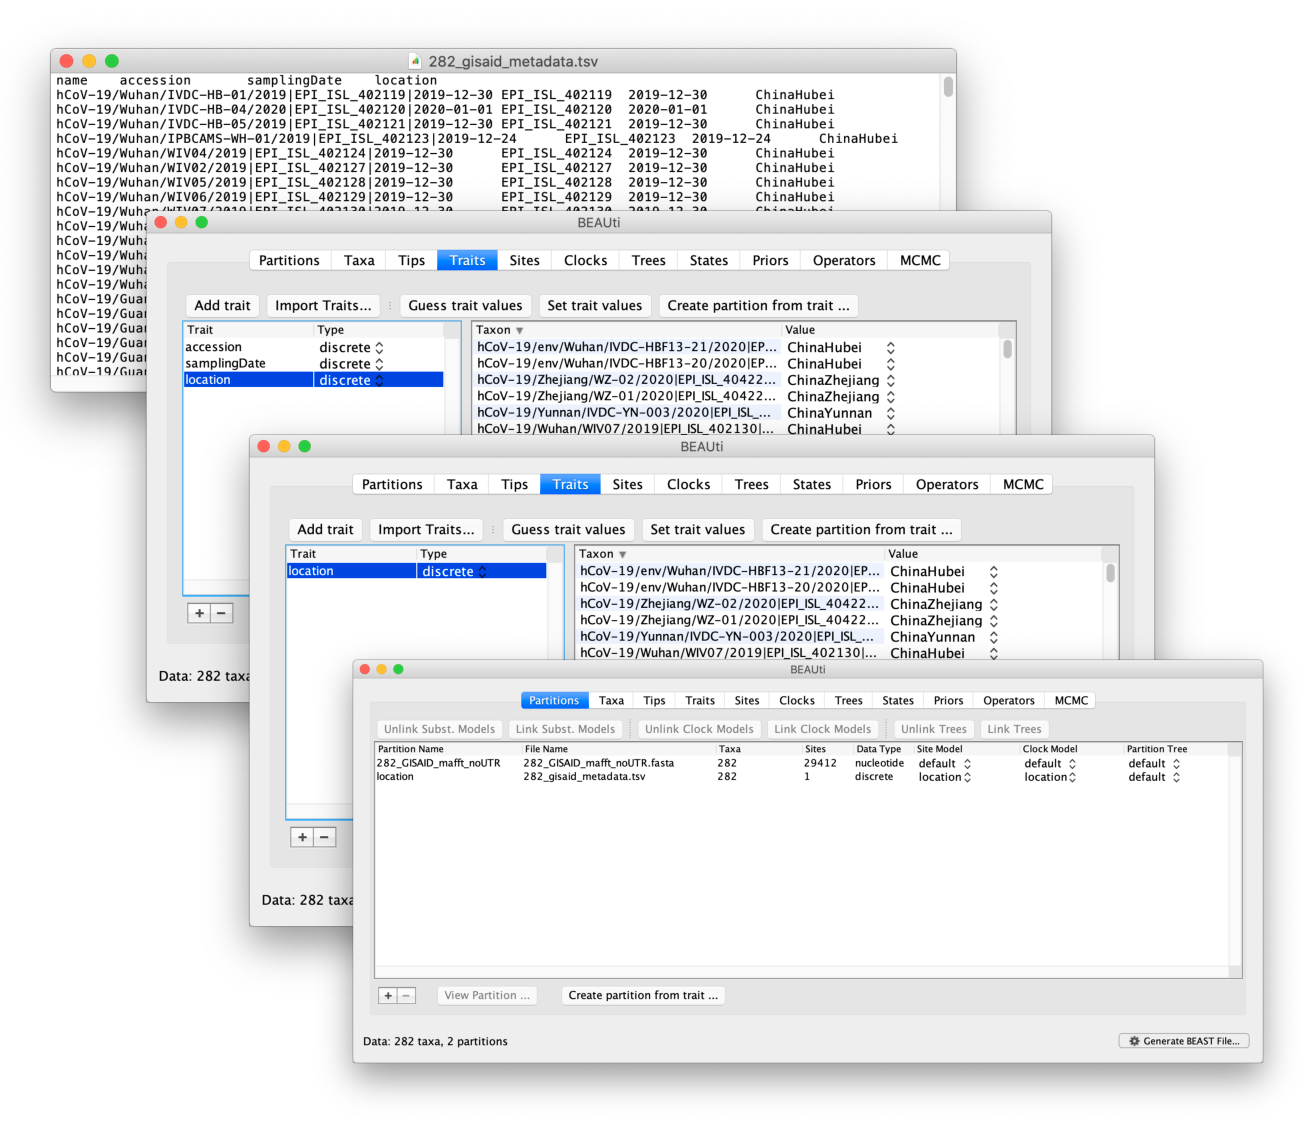
\includegraphics[width=1\textwidth]{figs/location_trait.pdf}
    \caption{Adding the sampling locations as a trait. From back to front: $i)$ tab-separated metadata file containing sequence names and sampling locations $ii)$ columns in the metadata file other than ``name" loaded as traits. $iii)$ traits different from ``location" removed from the analysis $iv)$ partition corresponding to the ``location" trait created.}
    \label{fig:location}
\end{figure}

\clearpage

4. Set up the nucleotide and trait substitution models\\

Click on the ``Sites" tab. Following \cite{travhist}, we will specify an HKY+$\Gamma$ nucleotide substitution model, and a GLM for the location trait.
Load the covariates by clicking on ``Setup GLM'' and ``Import Predictors'' (Figure \ref{fig:GLM}). In this example, we inform the rates of spread between locations using two predictors: a flight matrix containing air travel data between locations, and a distance matrix containing intra-continental distances. %GB: why is the distance matrix intra-continental while the flight matrix connects the locations? %SH: Not sure about this, my intuition is telling me it may be as a proxy to non-air travel, Philippe? %PL: indeed, I don't really see how transcontinental travel is by anything other than air travel. We can have many transcontinental transitions due to air travel, so making distance a poor predictor, while it could still be a reasonable one within continents (indeed as proxy to non-air travel).
Check the ``Log'' and ``Std'' boxes to log-transform and standardize the GLM predictors.\\

\ann{In this context, the terms `predictor' and `covariate' are used interchangeably.  
By default, each predictor name will be the same as the name of the file it originates from. Non-pairwise covariates can also be setup as origin and destination predictors in this window. Predictor files are comma-separated value (CSV) files formatted in two different ways depending on the nature of the predictor. For pairwise predictors, the CSV file is in the form of a square matrix with the different locations as column and row names alphabetically ordered, with rows denoting the origin and columns the destination. %GB: in the case of asymmetric matrices, are the rows the 'from' locations and the columns the 'to' locations? Best to mention here (it's not explicit in our beast.community tutorials either). %SH: Added.
For origin-destination predictors, the CSV file is in the form of a two column table with location names alphabetically ordered and predictor values.
You can also specify new predictor names by double clicking on each name, which allows you to enter a name of your choosing.
}

\begin{figure}[!ht]
    \centering
    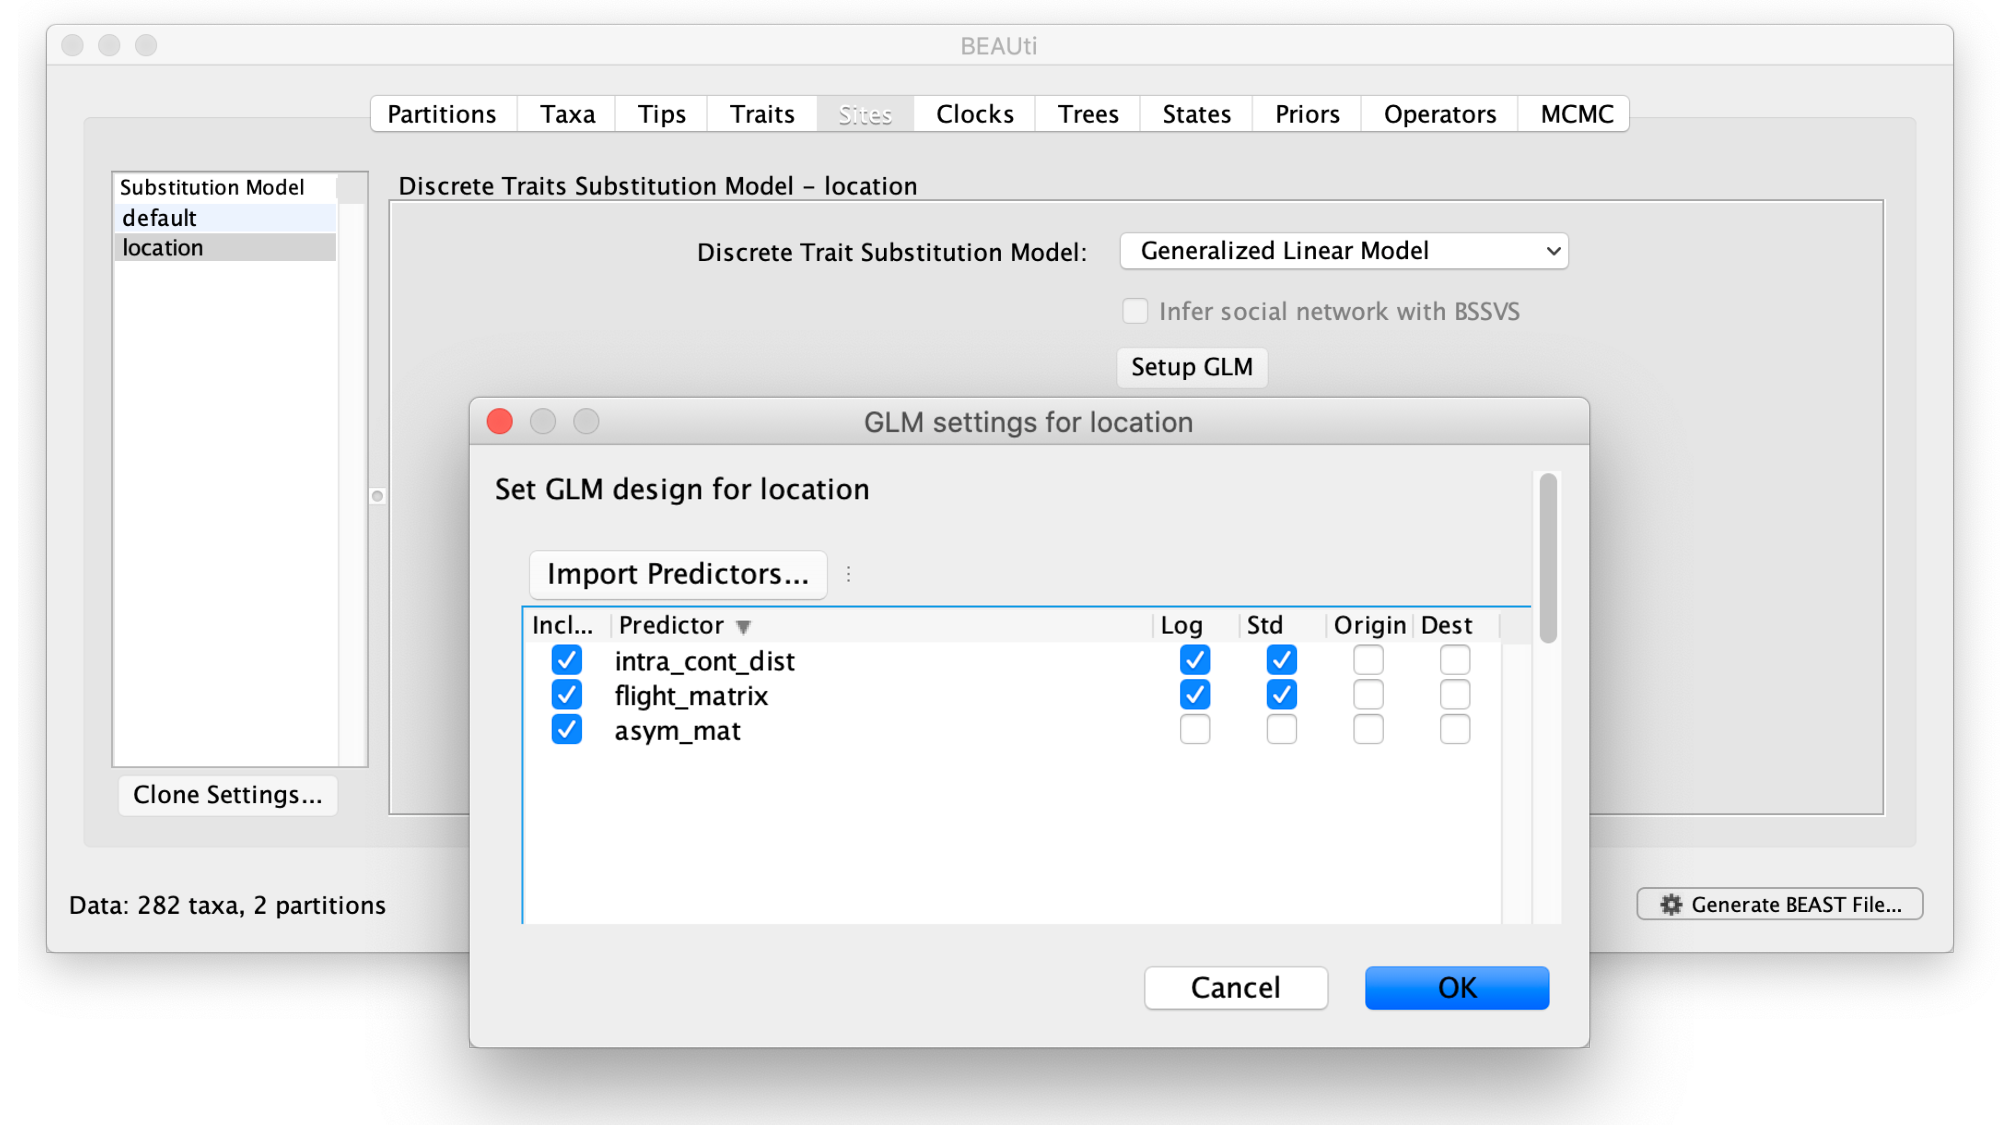
\includegraphics[width=1.0\textwidth]{figs/GLM.pdf}
    \caption{Setting up the predictors for the GLM-based spatial diffusion model. In this example, we load the air travel and intra-continental distance predictors, and log-transform and standardize them by checking the corresponding boxes.}
    \label{fig:GLM}
\end{figure}

5. Specify a clock model\\

Following the model specifications in \cite{travhist}, click on the ``Clocks" tab to specify a strict clock model for both the nucleotide and trait partitions.\\
\ann{BEAST analyses operate under the assumption of a molecular clock to estimate time-stamped phylogenies from the molecular sequence data and associated sampling times.
For this to hold valid, there needs to be sufficient temporal signal in the data (see the section \textbf{Critical parameters and troubleshooting}).
The presence of temporal signal in a data set can be assessed using TempEst \cite{tempest} and more formally tested using Bayesian Evaluation of Temporal Signal (BETS) \cite{bets}.
For more information on the different molecular clock models available in BEAST: {\upshape\url{https://beast.community/clocks}}}

6. Specify a demographic model\\

Click on the ``Trees" tab to specify the Tree prior. Following \cite{travhist}, we specify an exponential growth coalescent model parameterized with a growth rate parameter.
We refer to \url{http://beast.community/tree_priors} for a more detailed explanation on a subset of the available coalescent models in BEAST. \\

\ann{By default, BEAST will initialize the analysis with a randomly generated starting tree. It is also possible to start the analysis from a user-specified time-scaled phylogeny. This is usually done to reduce the burn-in time required for the tree topologies to converge. Specify a starting tree by clicking on ``Import Data" under the ``File" menu, to load a phylogenetic tree in Nexus format into BEAUti.}

7. Set up the ancestral state reconstruction for the location trait\\

Click on the ``States" tab and select the location partition. 
Check the ``Reconstruct state change counts" and ``Reconstruct complete change history on tree" boxes to save complete realizations of the spatial spread process on the output trees.
Be warned that this latter option might lead to large file sizes.\\

8. Specify the priors \\

Click on the ``Priors" tab. Following \cite{travhist}, we use default priors and only specify a Lognormal prior with \code{mu=0} and \code{sigma=10} for the effective population size (where\code{mu} and \code{sigma} represent the log-mean and log-standard deviation), and a Laplace prior with \code{mean=0} and \code{scale=100} for the exponential growth rate parameter.\\ %GB: please mention clearly which parameters of the lognormal distribution are meant with mu and sigma. %SH done.

\ann{BEAST aims to offer sensible default priors when informative prior information is unavailable, most of which can be considered largely uninformative. A wide range of prior distributions is also available to customize each analysis as needed.}

9. Set up the transition kernels \\

Click on the ``Operators" tab. Identify the tip-date sampling transition kernels in the table.
These have the description ``Uniform sample from precision of age of this tip".
The parameters associated with these transition kernels tend to converge rapidly and have good mixing (i.e. their effective sample size -- or ESS -- accumulates rapidly).
Decrease the weight of these operators to 0.25, but leave the weights of the other transition kernels at their default values, to sample these parameters less frequently so that the analysis gets to spend more time on estimating other parameters of interest.\\

\ann{Transition kernels (called ``operators'' in BEAST) are used to propose new values for each parameter being estimated during the analysis.
Different combinations of transition kernels can be used to fix certain parameters and customize the analysis as needed (e.g. estimating spatial spread on a fixed user-provided tree).}

10. Set up the MCMC options and generate the BEAST XML file\\

Click on the ``MCMC" tab. Set ``Length of chain" to 200,000,000 states and ``Log parameters every" to 100,000 states.
This will thin the MCMC results so that only 2,000 samples are collected by the end of the run.
Set your file name stem to generate the desired output file names (e.g. \texttt{282\_GISAID\_sarscov2}), and click on ``Generate BEAST File" to create the BEAST XML file for this analysis.\\

\ann{Thinning consists of storing only every $n$th sample from an MCMC analysis. This subsampling technique is done to decrease the autocorrelation in the samples collected and reduce the file size of the output. This is important since Bayesian phylogenetic analyses often require very long chains, and storing every single state would be prohibitive for file storage.}


\section*{PROTOCOL 3: PHYLOGEOGRAPHIC RECONSTRUCTION INCORPORATING TRAVEL HISTORY INFORMATION}

Phylogeographic reconstruction using DTA has been shown to be sensitive to spatiotemporal sampling bias. The ancestral reconstruction of locations will depend on the availability of samples from each location. In practice, this means that over/undersampling of sequences from a given location can greatly impact the ancestral locations being reconstructed. One way to mitigate sampling bias is through the incorporation of available travel history information from infected individuals. Travel history data can be used to correct for gaps in sampling by allowing for ancestral nodes to be in a given location even when molecular sequence data for that location are not available.\\

This protocol explains how augment a DTA analysis generated in BEAUti by incorporating individual travel history data.
In this example, we will use the XML file generated in Protocol 2 and modify it to include the available travel history data (See \cite{travhist} for more detailed information).
Importantly, BEAST requires its accompanying high-performance computational library for statistical phylogenetics -- known as BEAGLE \cite{beagle3} -- to be installed in order to optimise computational performance on a variety of hardware resources.

\subsection*{\textbf{\textit{Necessary Resources}}}
\subsubsection*{Hardware}
\hspace{0.5cm}Standard computer running Linux, MacOS, or Windows.

\hspace{0.5cm}CUDA-compatible Graphics Processing Unit (optional but recommended)

\subsubsection*{Software}
\hspace{0.5cm}Python v3.6+ with packages numpy and lxml

\hspace{0.5cm}BEAGLE v3+

\hspace{0.5cm}Latest BEAST jar file (v1.10.5) (provided with this protocol)

\hspace{0.5cm}\verb|add_travel_history.py| Python script (provided with this protocol)

\subsubsection*{Files}
XML file for a DTA+GLM analysis set up in BEAUti \\
Travel history metadata CSV file \\
Augmented covariate data files \\

\ann{Example files are provided in the repository {\upshape\url{https://github.com/hongsamL/travHistProtocol/tree/main/files/Protocol3}}. %GB: replace with actual github link. %SH fixed
The example in this protocol assumes an XML file for a DTA+GLM phylogeographic reconstruction with new travel history locations not present in the original BEAST XML file generated by BEAUti.
Covariate files augmented to include the new locations are thus required to accommodate for the increase in state space.}

1. Update the BEAST XML file to incorporate travel history data
\begin{verbatim}
python add_travel_history.py --xml 282_GISAID_sarscov2.xml
        --hist travel_metadata.csv
        --covariate augmented_flight_matrix.csv
        --covariate augmented_intra_cont_dist.csv
        --out 282_GISAID_sarscov2_travelHist.xml
\end{verbatim}

\ann{Although this example uses a DTA+GLM analysis, the\code{add\_travel\_history.py} script also works for symmetric and asymmetric DTA analyses. For such cases, run the same command without the\code{--covariate} flags. This script also requires for the travel history metadata to follow a specific format (Figure \ref{fig:travmeta}).
The metadata file is in CSV format and must contain the following columns: ``name"  (taxon name), ``travelHistory"  (travel location), ``travelDays"  (date of travel as days before to sampling date), ``priorMean"  and ``priorStdev"  
(prior specifications for the mean and standard deviation of a normal prior on travel dates when exact data are unavailable).}

\begin{figure}[!ht]
    \centering
    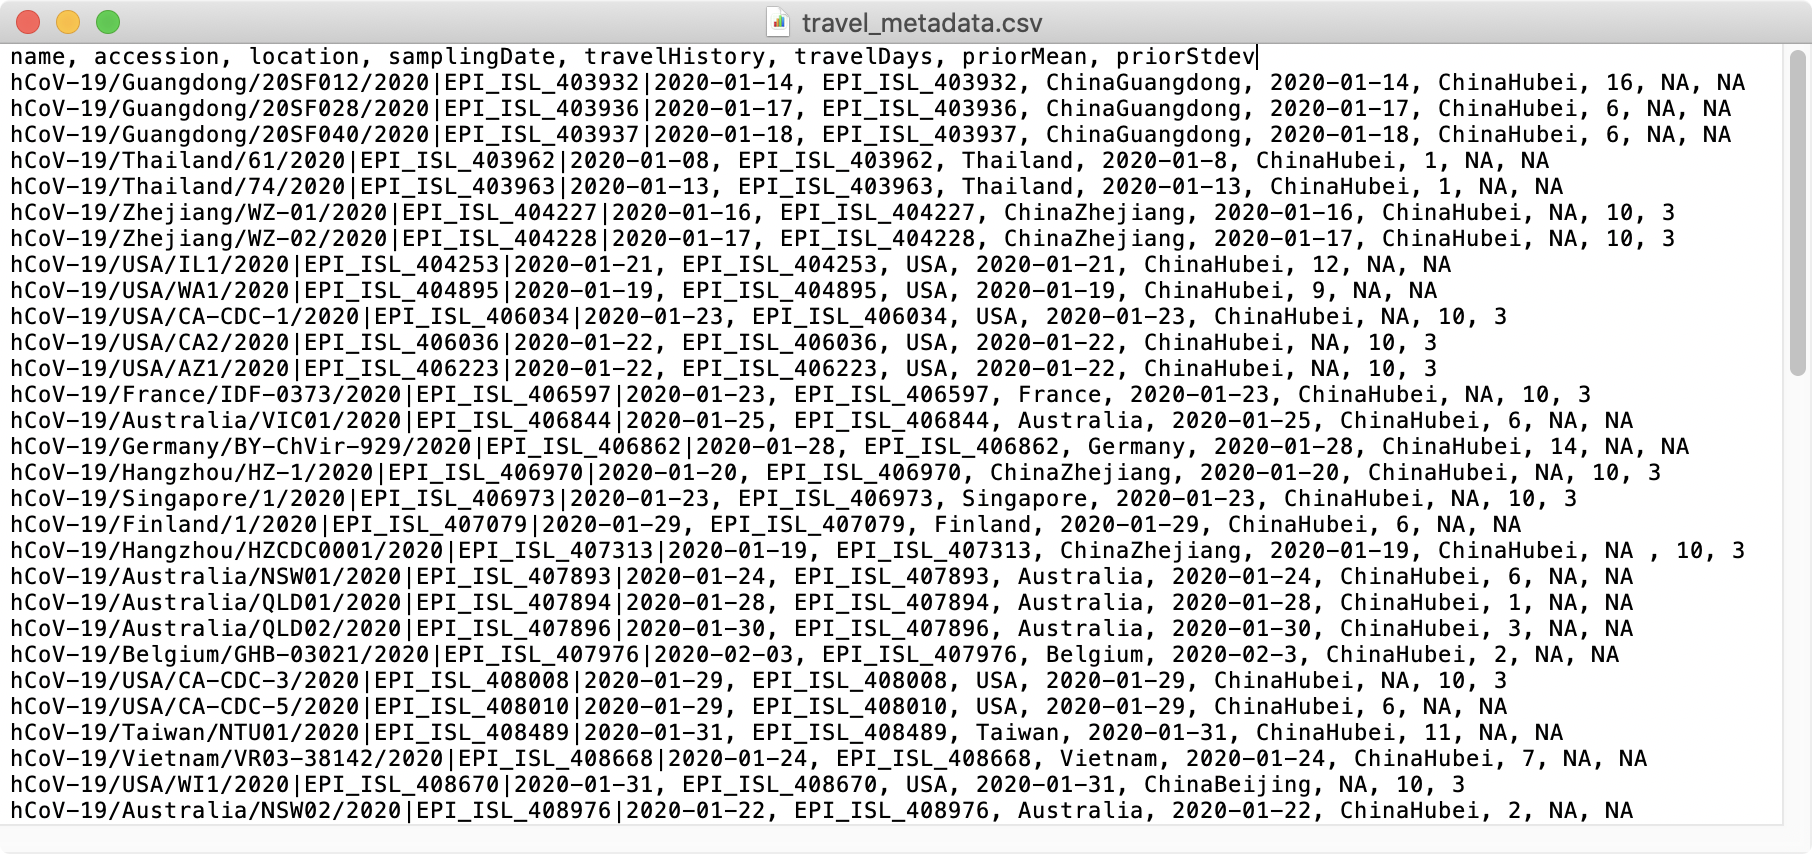
\includegraphics[width=0.99\textwidth]{figs/travelhist.png}
    \caption{Travel history metadata. The metadata file must contain the columns ``name", ``travelHistory", ``travelDays", ``priorMean" and ``priorStdev". Other columns can be included but will not be parsed to update the XML. For sequences where either exact travel dates are not available, we set the ``travelDays" column to \code{NA}, such that the MCMC samples from a range of possible travel dates with a Gaussian prior distribution of mean ``priorMean" (in units of days) and standard deviation ``priorStdev". For sequences were exact travel dates are available, we set the prior columns to \code{NA}.}
    \label{fig:travmeta}
\end{figure}

2. Run the updated XML file using BEAST
\begin{verbatim}
java -cp beast.jar dr.app.beast.BeastMain -seed 2020  
        -beagle_double	
        -beagle_gpu
        -save_every 1000000
        -save_state travelHist.checkpoint
         282_GISAID_sarscov2_travelHist.xml
\end{verbatim}

\ann{Here, we run BEAST on the command line using the latest build of BEAST. You can create your own beast.jar file by checking out and compiling the main branch of the \code{beast-mcmc} GitHub repository. We specify a starting seed with the -seed flag, and use the \code{-beagle\_cuda} flag to accelerate the likelihood computations using a GPU (only applicable if you have a powerful GPU with sufficient double precision -- or FP64 -- compute performance available).
This option is recommended when available, as using a GPU reduces runtime by accelerating likelihood computations when performing phylogeographical analyses on large datasets.
Be sure to check the technical specifications of the GPU you want to use; you'll ideally want at least 3 TFLOPS FP64 performance.
We also take advantage of the BEAST checkpointing functionality \cite{onlineBEAST} to save a snapshot of the MCMC run into the travelHist.checkpoint file every 1,000,000 states.
This allows us to resume the analysis from the checkpoint in case the run becomes interrupted, or more iterations are required than initially anticipated.}


\section*{PROTOCOL 4: VISUALIZING INDIVIDUAL-SPECIFIC SPATIAL TRAJECTORIES}
\subsection*{\textbf{\textit{Necessary Resources}}}
\subsubsection*{Hardware}
Standard computer running Linux, MacOS, or Windows. 

\subsubsection*{Software}
%\hspace{0.5cm}BEAGLE v3+

\hspace{0.5cm}Latest BEAST jar file (v1.10.5) (provided with this protocol)

\hspace{0.5cm}R with package MarkovJumpR

\subsubsection*{Files}
Trees output from a BEAST travel history DTA+GLM analysis \\

1. Extract all Markov jump histories for an isolate of interest
\begin{verbatim}
java -cp beast.jar dr.app.tools.TaxaMarkovJumpHistoryAnalyzer 
        -taxaToProcess "hCoV-19/Brazil/SP-02/2020|EPI_ISL_413016|2020-02-28" 
        -stateAnnotation location
        -burnin 100
        -msrd 2020.1748633879781
         282_GISAID_GLM.location.history.trees EPI_ISL_412975_MJhist.csv
\end{verbatim}

\ann{The BEAST jar file packages a number of standalone applications that can be accessed by using the -cp flag when calling Java from the command line.
Here, we use the TaxaMarkovJumpHistoryAnalyzer application to extract all Markov jump histories for isolate EPI\_ISL\_413016, into a CSV file.
This application takes a trees file with complete state change history as an input (which is being generated by running the XML constructed in the protocol), and outputs all spatial trajectories for a selection of taxon/taxa.
We specify the desired taxon labels through the\code{-taxaToProcess} flag, and specify the annotation name of the discrete trait that was reconstructed using \code{-stateAnnotation}.
We can also remove a number of trees corresponding to the burn-in using the \code{-burnin} flag, and scale the output results to reflect chronological time instead of node heights using the \code{-msrd} flag by specifying the most recent sampling date.
An example output file can be found in {\upshape\url{https://github.com/hongsamL/travHistProtocol/tree/main/files/Protocol1}}}

2. Load spatial trajectories into R
\begin{verbatim}
library(MarkovJumpR)
spatial_paths <- loadPaths(fileName = "EPI_ISL_413016_MJhist.csv")
\end{verbatim}

3. Inspect spatial trajectories reconstructed
\begin{verbatim}
spatial_paths$minTime
\end{verbatim}
yields the earliest time along a spatial path across all trees
\begin{verbatim}
2019.892
\end{verbatim}


To look at the frequency of locations visited across all spatial paths we type
\begin{verbatim}
loc_freq <- table(spatial_paths$paths$location)
loc_freq[order(loc_freq,decreasing = T)]
\end{verbatim}
which yields a frequency table of locations in descending order
\begin{verbatim}
         Italy         Brazil     ChinaHubei    Switzerland        Finland 
           444            437            436             85             23 
  ChinaBeijing             UK      Australia        Germany            USA 
             9              8              7              6              6 
        France      Singapore          Spain  ChinaHongKong          Japan 
             5              5              5              4              3 
   Netherlands         Sweden        Vietnam ChinaGuangdong  ChinaShandong 
             3              3              3              2              2 
    NewZealand       Thailand        Belgium       Cambodia         Canada 
             2              2              1              1              1 
ChinaChongqing    ChinaFujian    ChinaYunnan          India           Iran 
             1              1              1              1              1 
        Mexico          Nepal       Portugal     SouthKorea         Taiwan 
             1              1              1              1              1     
\end{verbatim}

In this example, we see that Italy, Brazil, ChinaHubei and Switzerland appear most commonly across the spatial paths. \\

4. Set up plot colors \\

We here specify four colors of choice corresponding to the four locations of interest that make up the spatial trajectory of isolate EPI\_ISL\_413016.

\begin{verbatim}
locations <- c("ChinaHubei","Italy","Brazil","Switzerland")
locationColors <-c("#E3272F","#31B186","#931ECF","#C695BD")
locationMap <- data.frame(location = locations,
                position = c(1, 2, 3, 4))
locationMap$color <- sapply(locationColors,as.character)                
\end{verbatim}

5. Set up plot labels
\begin{verbatim}
dateLabels <- c("01-Dec-19", "15-Dec-19", "01-Jan-20", "15-Jan-20",
                "01-Feb-20", "15-Feb-20", "01-Mar-20")
\end{verbatim}

6. Plot path spatial trajectories
\begin{verbatim}
plotPaths(travelHistPaths$paths, locationMap = locationMap,
        yJitterSd = 0.1, alpha = 0.1, minTime = spatial_paths$minTime,
        addLocationLine = TRUE,
        xAt = decimal_date(dmy(dateLabels)),
        xLabels = dateLabels,
        mustDisplayAllLocations = TRUE)
\end{verbatim}

\begin{figure}[!ht]
    \centering
    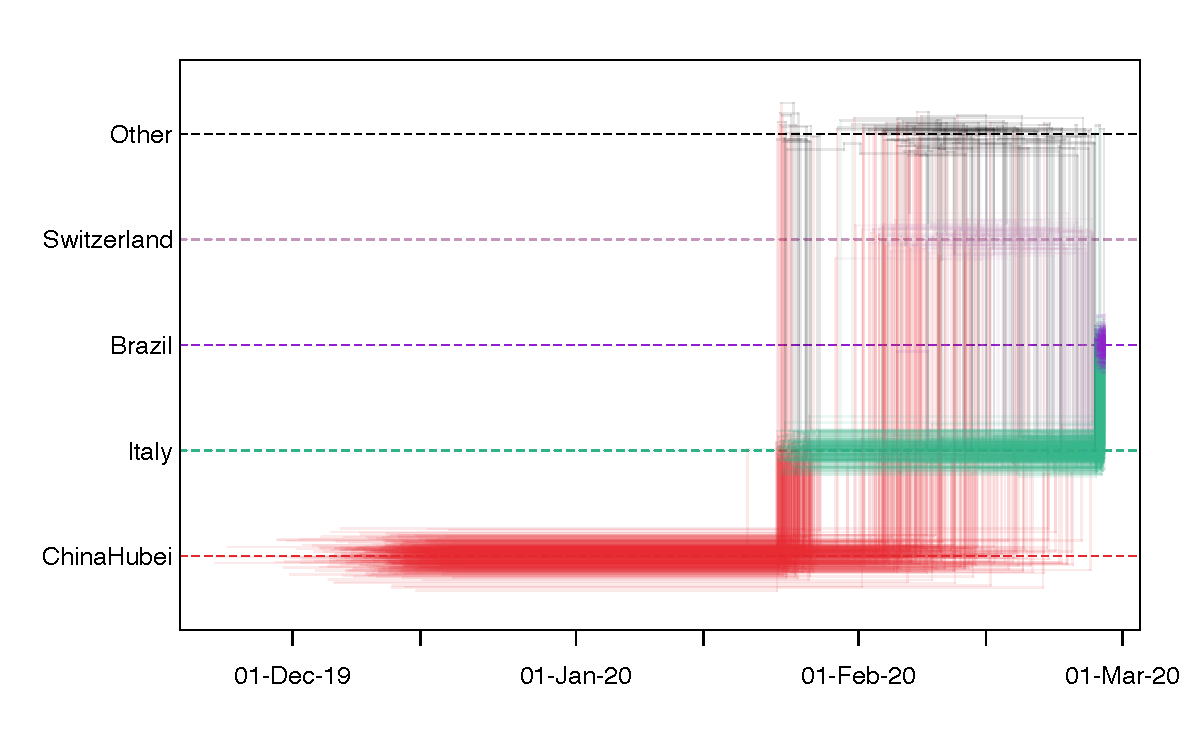
\includegraphics[width=1.0\textwidth]{figs/travel_trajectory.pdf}
    \caption{Spatial trajectory plot of isolate EPI\_ISL\_413016. The plot depicts the posterior spatiotemporal ancestral transition history for a single isolate. Each line represents a single Markov jump history in the posterior distribution. The time spent in each location is denoted in the horizontal dimension, and transitions between two locations are depicted with vertical lines. The relative density of lines reflects the posterior uncertainty in location state and transition time between states. Here we see that the most supported ancestral history for isolate EPI\_ISL\_413016 is that of an origin in Hubei, with a jump into Italy late January, and an introduction into Brasil close to March 1st.}
    \label{fig:trajectory}
\end{figure}


\section*{GUIDELINES FOR INTERPRETING RESULTS}

The BEAST software package offers a flexible approach for combining demographic, molecular clock, nucleotide and trait evolution models to infer time-scaled trait-annotated phylogenies.
BEAST employs Bayesian inference through MCMC to sample trees and all of the model parameters from the joint density (often simply called the posterior).
Protocols 2 and 3 show how to set up the different models and run the corresponding BEAST analyses to collect samples from the posterior.
The phylogenetic trees that are sampled from the posterior are stored in a\code{.trees} file and samples of the model parameters are stored in a\code{.log} file.
Here we present some of the standard applications that are commonly used to interpret the output that BEAST generates.

\subsection*{Assessing convergence}

The MCMC sampling strategy is to construct a Markov chain that (eventually) converges to a stationary distribution, which is the joint density in the case of Bayesian inference.
Given enough time we know that the chain will converge, but it may take considerable time for this to happen. We can visually assess the convergence of a BEAST run by inspecting the sampled parameter values across an MCMC analysis.
To do so, we can load a\code{.log} file into Tracer (\url{https://beast.community/tracer}, \cite{tracer}), %GB: add citation for Tracer publication %SH: done
 and visually inspect the trace plot, which shows a time series of the parameter values sampled throughout the analysis.
A detailed guide on how to use Tracer can be found at \url{https://beast.community/tracer_convergence.html}

\subsection*{Effective sample size and parameter estimates}

Loading a .log file in Tracer will also show the effective sample size (ESS) values and estimates for each model parameter.
Note that ESS values are only defined for continuous parameters that are being estimated.
A characteristic of inference through MCMC is that the samples collected tend to be correlated.
This in turn poses a challenge, since having a large number of samples does not guarantee a considerable reduction of the uncertainty in our posterior estimates.
A way to control for this is to look at the ESS value associated with parameter estimation.
The ESS of a parameter sampled from an MCMC method is the number of effectively independent draws from the posterior distribution that the Markov chain is equivalent to.
ESS values will increase as more and more samples are collected by the sampler.
Higher ESS values will result in more precise posterior estimates but require higher computational resources.
Tracer will automatically calculate the ESS for all parameters part of the log file, and flag values above 100 (acceptable) and 200 (ideal).

\subsection*{Summarizing trees and phylogeographic estimates}

Individually inspecting every tree from the posterior obviously constitutes an impractical way to interpret the MCMC results. We are thus required to summarize the distribution of trees sampled as a point estimate with associated uncertainties. The TreeAnnotator application in BEAST enables creating a maximum clade credibility (MCC) tree to summarize the sampled trees for this purpose. For every tree in the distribution, a posterior clade probability for each node (i.e. the support for a node) is calculated by computing the frequency of the clustering that is defined by the node in question. The MCC tree is then defined as the tree that maximizes the product of the posterior clade probabilities across the tree. Instructions on how to use TreeAnnotator can be found at \url{beast.community/second_tutorial}. \\

In some data sets, the posterior support for all nodes in a tree is such that many topologies do not end up represented in the MCC tree.
When that is the case, a point estimate of a tree is unable to capture the diverse phylogeographic histories compatible with the data. Protocol 4 allows us to inspect individual spatial trajectories by summarizing across all possible phylogenetic ancestries in the joint density. Each spatial trajectory in the joint density is represented by a stepwise curve, where vertical lines represent transitions between two locations, and horizontal lines time intervals where the pathogen remains in the same location. The relative density of lines reflects the posterior uncertainty in spatiotemporal ancestry.

\begin{multicols}{2}

\section*{COMMENTARY}
\subsection*{Background Information}

Models for phylogeographic inference can be broadly categorized into two classes or types, depending on the assumptions used to model the spatial spread of a pathogen.
Structured coalescent approaches model movement in terms of a migration matrix, and relate migration rates with a location's population size, which involves population size dynamics having to be estimated for each location \cite{basta,mascot}.
On the other hand, diffusion approaches consider sampling locations as observed traits independent from the tree-generative process, and model movement across space using a continuous-time Markov chain (CTMC) \cite{dta,rw}. 
While structured coalescent approaches are theoretically a more robust, the lack of computationally efficient implementations (especially for larger datasets) has made diffusion methods more widely adopted.
Currently, BEAST v1.10.5 focuses on providing phylogeographic inference using CTMC models in the case of discrete location data.

Diffusion models for phylogeographic inference can be further categorized depending on the spatial resolution being considered.
Discrete locations are modeled using discrete trait analysis (DTA), with transition rates between locations in the form of a CTMC matrix analogous to those used to model nucleotide substitutions \cite{dta}.
In contrast, continuous locations are modeled using Brownian diffusion-based random walk models \cite{rw}.
Much of the genomic data collected has a spatial resolution coarser than latitude and longitude, which makes DTA the only practical approach to study the spread of an epidemic. 

Under the DTA formulation, movement between K discrete locations is parameterized in terms of a $K \times K$ infinitesimal rate matrix $\Lambda$, where $\Lambda_{ij}$ is the instantaneous movement rate from location $i$ to $j$. This model has been extended to allow for symmetrical and asymmetrical transition rates, and uses Bayesian Stochastic Search Variable Selection (BSSVS) to limit the number of rates to only those that adequately explain the phylogenetic diffusion process. An alternative formulation of this model parameterizes the rate matrix using a generalized linear model \cite{glm}. Here, the transition rates are defined as a linear combination of $P$ of potential explanatory predictors $(x_{ij1}, \dots, x_{ijP})$, with corresponding coefficients $(\beta_1, ..., \beta_P )$ and indicator variables $(\delta_1, ..., \delta_P )$ such that log$(\Lambda_{ij}) = \sum_{p=1}^P \beta_p \delta_p x_{ijp}$. This model specification allows us to use BSSVS to explore the space of $2^P$ predictor combinations and obtain a posterior probability on the indicator variables to determine the support for inclusion of each predictor in the model.

Incorporating individual travel history data does not require the use of a GLM and can be added to both symmetric or asymmetric DTA \cite{dta}) by augmenting the available dataset to include ancestral nodes associated with a known state but not necessarily with a known sequence \cite{travhist}.
These ``ghost samples'' enable exploiting individual travel cases for which molecular sequence data could not be obtained.
Ambiguous ancestral locations can also be allowed by integrating over the all possible locations with equal or user specified weights \cite{ambig}.
An example would be the case where an individual traveled to multiple locations prior to being sampled.
Given that the individual could have gotten infected in any of the visited countries, we can integrate this uncertainty by marginalizing over all potential locations for the unsampled ancestor when performing phylogeographic inference.


\section*{CRITICAL PARAMETERS AND TROUBLESHOOTING}

A critical assumption for any BEAST analysis is that the data set under consideration constitutes a sample from a measurably evolving population (MEP). MEPs \cite{mep1,mep2} refer to time-stamped sequence data where a sufficient amount of molecular evolution has occurred throughout the sampling period to establish a statistical relationship between genetic divergence and time. A data set conforming to this criteria is said to contain sufficient temporal signal. A lack of temporal signal will ultimately result in flawed analyses with unreliable divergence time estimates. Popular ways to assess temporal signal include doing a root-to-tip regression of genetic divergence and sampling times on a maximum likelihood tree \cite{tempest} and permutating tip date labels through date-randomization \cite{tipdate}. Recently, a formal way to assess temporal signal has been developed under a Bayesian framework using model comparison through Bayes factors \cite{bets}. In cases where the temporal signal is deemed insufficiently strong, one can resort to adding more data to increase temporal coverage or using prior knowledge to inform the molecular clock rate or the time to the most recent common ancestor.

Another commonly encountered issue is that of low ESS values for parameters relevant to the analysis. At the end of a BEAST analysis, some parameters may have much higher ESS values associated to them compared to others. One way to increase the ESS values of a parameter is to decrease the weight of other parameters that have been able to attain sufficiently high (or very high) ESS values to increase the sampling frequency of the (problematic) parameter of interest (e.g. Protocol 2, step 9). Other ways to obtain more samples -- and as a result increase the ESS value -- include increasing the MCMC chain length and combining the output of multiple independent BEAST analyses, i.e. analysing the same XML file using BEAST but with different starting seeds.


\section*{SUGGESTIONS FOR FURTHER ANALYSIS}

This section is optional but I'm open for suggestions.



\bibliographystyle{apalike}
\bibliography{protocol}

\end{multicols}

\end{document}
